%% Author: Sakhile Masoka (851667@students.wits.ac.za)
%% Homepage: https://github.com/smasoka/CODE-RADE-project/tree/sakhile-project
%% Reference: 
\RequirePackage{ifpdf}
\documentclass [titlepage,11pt]{article}

\usepackage{witsa4}
\usepackage{times}
\usepackage{enumerate}
\usepackage[inline]{enumitem}
\usepackage{graphicx}
\usepackage{subcaption}
\usepackage{afterpage}

\usepackage{url}
\usepackage{natbib}

\usepackage[center]{titlesec}

\input{natbib-add}
\bibliographystyle{named-wits}
\bibpunct{[}{]}{;}{a}{}{}


\title{\Huge Continuous Delivery of Research Application in a Distributed Environment \\\medskip Research Proposal}
\author{Sakhile Masoka (851667@students.wits.ac.za)\\Witwatersrand University}

\begin{document}
\maketitle



% Provides Context
% Idea Of Own Contribution
% What Will Be Done
% How It Will Be Done
% Can Be Read Independently
% Measures (metrics) Used and Results Very Good
\begin{abstract}
One of the aims of e-Infrastructures is to provide easy access to powerful computational and data platforms, to as many eligible users as possible. The South African National Grid (SAGrid), as part of the National Integrated Cyberinfrastructure System is no exception. While access to the users is being simplified greatly by the adoption of science gateways and identity federations, the community of application developers and technical support in scientific collaborations does not yet have an easy way to integrate these applications in the first place.\\

SAGrid has identified this as a gap in the services it provides and has developed a solution to the issue of easily integrating new applications into the infrastructure in a fast, flexible, distributed and reproducible way. Using existing tools and services, SAGrid has defined a simple set of tests which applications need to pass in order to be considered valid for the infrastructure.\\  

The proposal is to use a continuous integration platform, Jenkins, to encode these tests automatically. Critical to the process is the Inter-operability between source code repository, automated build system, artifact creation and a content delivery system to site infrastructures to sustain the system. These will be tested using scientific applications, namely GADGET, Quantum Espresso and common based frameworks applications such as R and Python.

\end{abstract}


\tableofcontents{}
\listoffigures
\newpage

% Introduces General Problem Area
% Introduces Specific Problem Area
% Research To Be Followed
% Provides Idea About Expected Results
% Provides Idea Of Research Contribution
% Correct Level Of Detail? 
% Provides Structure to Rest Of Document

% One of the aims of e-Infrastructures is to provide easy access to powerful computational and data
% platforms, to as many eligible users as possible. The South African National Grid (SAGrid), as part
% of the National Integrated Cyberinfrastructure System is no exception. While access to the users is
% being simplified greatly by the adoption of science gateways and identity federations, the community
% of application developers and technical support in scientific collaborations does not yet have an easy
% way to integrate these applications in the first place.
\section{Introduction}

e-Science  is a computationally intensive science that is carried out in highly distributed network environments, or science that uses immense data sets that require grid computing, the term sometimes includes technologies that enables distributed collaboration, such as the Access Grid. \citep{escience}. This leads to working definition of e-Infrastructures as networked tools, data and resources that support a community of researchers, broadly including all those who participate in and benefit from research. e-Infrastructures include services as diverse as the physical supply of backbone connectivity,single- or multi-purpose grids, supercomputer infrastructure, data grids and repositories, tools for visualization, simulation, data management, storage, analysis and collection, tools for support in relation to methods or analysis, as well as remote access to research instruments and very large research facilities, according to the eResearch2020 Final Report \citep{eresearch}.\\ 

The National Integrated Cyberinfrastructure System (NICIS) is a framework of an integrated system for cyberinfrastructure in South Africa, which includes pillars of data, computations and network infrastructure. South African Grid (SAGrid) is part of the South African National Research Network (SANReN), which is one of the network pillars on NICIS. SAGrid carries the mandate to enable anyone, with the right credentials to access the Cyberinfrastructure (data,compute,software,metadata, support, etc services) and to provide tools for collaboration and research \citep{nicis}. \\

% The General/Specific Problem and Solution
In this mandate, user access has seen great improvement through the introduction of science gateway and identity federations. Science Gateways \citep{scienceG} are community developed set of tools, applications, and data collections that are integrated through a portal or a suite of applications. These gateways enable entire communities of users with a common scientific goals to use digital resources through a common interface, even when such resources are geographically distributed. SAGrid provides access through the Africa Grid Science Gateway \citep{africa_gateway}.\\

Science gateways require federated identities to enable secure access to different users having different roles and privileges. Formally, Federated identity is the means of linking a person's electronic identity and attributes, stored across multiple distinct identity management systems \citep{federation}. SAGrid provides federated credentials through Istituto Nazianale di Fisica Nucleare (INFN) Certification Authority (National Institute for Nuclear Physics in Catania) \citep{identity}. Through the joint work of TENET and SANReN, a Federated Identity Management system is currently being developed and operated on South Africa. \\

This leads to the last challenge in the mandate where the community of application developers and technical support in scientific collaborations does not yet have an easy way of integrating applications to site infrastructures. The current workflow of finding source codes and recursively compiling and fixing dependencies manually consumes a lot of time. Without an easy process to achieve this, latest and relevant applications are not ported, which leads to users to lack interest in leaving their traditional cluster environment to grid open science. basically, what users want is an \emph{amazing} infrastructure, highly trained support stuff and a variety of applications to chose from. \\

SAGrid has proposed a better worklfow. Scientists propose an application they wish to use. Then what follows are
defined tests which applications need to pass in order to be considered valid for the infrastructure. Questions like can the application be compiled are answered. Using existing tools and services, the recursive process of compiling and solving for dependencies can be automated using continuous integration platforms. Combined with continuous delivery platforms, applications can be easily delivered to sites. \\ 

This research proposal aims to look at the methodologies and the platforms tools to configure these tests and automate them leading to better workflows. The greater goal is to lower the barrier to entry to the grid or cloud infrastructure, have a way to prove to resource providers that application will run on their environment, be able to manage application lifecycle across multiple versions, architectures, configuration and lastly deliver this applications to as many sites as possible.  The results will also lead to developing insights necessary to provide best-practice guidelines to future (platform and application) development and operation of the services, especially related to optimisation and automation procedures. \\

% Structure of the paper
The paper is structured as follows:Section 2 describes the problem statement in greater detail, motivation and the literature review. Section 3 looks into the research aim, answering the research question the paper aims to prove. Section 4 describes the methodology, the theory behind the intended implementation, the description of the software platform, and the application software. Section 5 is the proposed actual work to be done with time-lines. Section 6 discusses the intended results and conclusion. \\

% Provides Detail On Specific Problem Area
% Level Of Engagement With Research Literature
% Level Of Understanding Of Problem Background
% Contains Adequate And Relevant References 
% Contains Relevant Ideas, Concepts, etc., From References
% Relates Background Material And Related Work To Research Question
% Research Aim/Question Justified In Terms Of Past Research

% SAGrid has identified this as a gap in the services it provides and has developed a solution to
% the issue of easily integrating new applications into the infrastructure 
% in a fast, flexible, distributed and reproducible way.
\section{Background}

In this section, a problem statement is described along with the solution motivation. A few concepts and tools are introduced that will be covered more in detail in the later sections. I also cover the literature review, discussing the previous works (developed softwares) on application deployment by the grid community. 
% Detail description of the problem statement
\subsection{Problem Statement and Motivation}

% Explain how the applications are installed? 
As mentioned on the Introduction, Grid applications are installed by hand on each grid site where the application is needed. An operations team member develops a script, specifying the installation process, standard error and output for logging and output sandbox for retrieving the standard files. A job submission is launched with the script to the site infrastructure. If the job is successful, the site is has to be tagged, publicly declaring that jobs requesting this application can be sent and accepted. These tags are usually sent via the script. \\

This process has some flaws, one being there is a major overhead, if the same application is requested in a number of sites, many scripts and job submissions have to be created. Since sites are configured differently, installation procedures will be different. This is caused by different configured variables, different configured paths, dependencies, compatibility with different versions etc. This requires the application scientist to know a great deal about the infrastructure where the application is being installed. Since application scientist are not site administrators, this becomes a big communications problem. \\

A member of the operations team doing the work actually causes a porting bottleneck since its always a "few to many" relationship, so the community at large suffers. Prioritising porting requests then depends on the knowledge of the expert about the application and the site. The bottleneck is also caused by changes in the middleware stacks, which often requires new procedures and dependencies to make the same application compatible again. And another when sites gets upgraded with new architectures like GPGPU or ARM. To name these issues in a simple format, \begin{enumerate*}[label=\itshape\alph*\upshape)]
\item Applications are not centrally managed.
\item There are Dependency complications.
\item For each step in the process, manual intervention is needed by either the application scientist or the site administrator.
\end{enumerate*} \\

To solve these issues, restructuring is needed. Distribute the efforts but centralise the tools. Infrastructure like Github brings numerous advantages like enabling collaborations. Instead of operation members only, a large number of people can offer code contributions in a secure environment. With central tools, applications are managed in one place. This allows for a complete list of requested application for anyone to tackle and progress is easily seen and tracked. \\ 

Site administrators can configure secure permissions, ports etc without worrying about if a certain job is an installation and will require special access or not. Dependency complexity is solved by packaging every needed component in an installation and guarantee successful builds. Since these builds are a complete package (completes artefacts), the installations are platform independent. One installation will work of multiple sites. To properly make this solution work, a delivery system is needed that will transport all applications to sites. Site infrastructures subscribe to delivery repository and  deployment is made easy and manageable. \\

The proposed solution is integrated, from application development to application deployment, all steps are linked together. Its fast, all steps are automated together, duplicate work is eliminated, communication is open through collaborations and allows administrators either site or application to focus on their work, not overlapping. There is flexibility in the sense that firstly it scales, secondly its adaptable to all grid communities and thirdly, changes in site infrastructures has little affect on deployment. Lastly, using containers, the solution produces artefact's (installation files) which can be used anywhere. This solution is based on Development Operations, Continuous Integration and Continuous Delivery methodologies. On Section 4 these are discussed with their own tools. \\

% Literature Review on CODE-RADE 
\subsection{Literature Review }
Finding better ways to deploy applications on distributed infrastructures has been a concern for a number of years and various software solutions have been introduced to the community. Goscinski and Abramson \citet{wojtek05} developed an automated application deployment with a user-oriented approach called Distributed Ant, which provides a simple, scalable and secure deployment service and supports a simple procedural deployment description. DistAnt supports definition and deployment of application dependencies, infact the article cited here was to demonstrate that \emph{DistAnt enables deployment of a complex native application over an uncharacterized heterogeneous grid, assuming nothing about grid resources.} \\

How DistAnt is designed solves some of the deployment issues. There are description tasks that handles application description, Deployment tasks provides means of transporting files to remote hosts and Actions tasks that performs actions like executing procedures that unpacks, builds, install and configure application on remote hosts. This deployment system proved to be significant as users were able to deploy with only minimal resource knowledge, which is important in a dynamic grid environment, where resources are added and removed on a regular basis,particularly e-Science where scientists use computational resources opportunistically. \\

ADEM, Automating Deployment and Management of Application Software is another solution introduced to the community at a later stage \citep{zheng09}. Faced with similar issues as many Grid sites of performing deployment and management manually, which is error-prone and does not scale well large sites, this collaborative effort was born from China and USA. The developers acknowledged the previous work that was done, including DistAnt, but distinguished they software by stating that their research is focused on fully automating the process of deployment and management of real, domain-specific application software on the Open Science Grid and other Globus-equipped grids such as TeraGrid \footnote{TeraGrid was an e-Science grid computing infrastructure combining resources at eleven partner sites. The project started in 2001 and operated from 2004 through 2011.}. \\

ADEM automates dynamic collection of grid site resource and service contact information needed for application deployment, and can be adapted to different build approaches, such as prebuild and dynamic build. With the prebuild function, users do not need to compile their source code on every grid site. Prebuilt code, source code and dependencies are all stored on a repository that is accessible Grid site. This very idea of online repositories is the bedrock of continuous delivery, a design principle discussed later in this paper. 

A more recent take to offer a solution is ADAPT, a metadeployment system that manages and uses already existing deployment mechanisms that builds application from source code, and execution automation regardless of a selected target site and approaches heterogeneity using alternative recipes created for situation-specific cases \citep{slawinski14}. The software design stems from the steps a normal user will follow when faced with installation errors to seek aid from the community by using question-and-answer websites. The software has a tool to automatically detect deployment issues and reacts by deploying needed software or fix targets configurations. This approach is different from the rest as its doesn't package the application with its dependencies, but solves them as they arise. \\

% They chose to design these software from scratch. 
The design of these software platform differs, but they all have common components that are viewed necessary to build a fully working deployment system. They all have a deployment model which makes use of a repository to store and transport installation files and dependencies. These are either mounted on grid sites like ADEM, or use transportation protocols to copy files from repositories to sites when needed like DistAnt. There is a descriptive model in a form of descriptive language to specify installation procedures. And lastly, there is a execution model which provides execution mechanism on remote sites. A more interesting model is the ADAPT's, as its able to go on a recursive loop, that performs a series of autonomic error detection and repairs. Now these common components give directions to how a desired deployment system should look like and behave. \\

Now that we have reviewed some of the previous work done on application deployment on distributed environment, the next sections will explore in more details the design principles, as a result from this review and the technologies we propose to use. These will be the base of our research aim which is discussed in the next section.

% Has Presented Research Hypothesis/Focused Research Question
% Has Clearly Stated Hypothesis/Research Question
% Hypothesis Can Be Tested And Research Question Can Be Answered

% The specific problems we aim to address in this limited-scope project are those of automation and
% distribution. Specifically How far is it feasible to automate the build steps in order to produce high-quality, 
% re-distributable artifacts ?
% How are dependencies of applications to be managed in various configurations ?
% How can Linux containers be used to distributed these artifacts to remote sites with the minimum
% intervention necessary by site administrators
\section{Research Aim}
The specific problems this project aims to address are those of automation and distribution with the following questions (and their descriptions).  \\
% A mention of Jenkins and Docker
\begin{description}

\item \textbf{How far is it feasible to automate the build steps in order to produce high-quality, re-distributable artifacts?} Can automating every build step results into producing high quality artifacts? Another question is, can all the build steps be automated or some manual testing will still be needed? For this question, the project will explore the pipeline of delivering a scientific application in a distributed infrastructure by looking into software development disciples namely \emph{Continuous Delivery} \cite{delivery15} and \emph{Continuous Integration} \citep{fowler06}. Both these disciples stem from DevOps \citep{wikiOps}, a software development method  stresses communication, collaboration, integration, automation, and measurement of cooperation between software developers. Specifically, Jenkins will be highlighted as the best software platform to possibly to explore, implement and answer this question. \\

\item \textbf{How are dependencies of applications to be managed in various configurations?} With different scientific applications having different degrees of complex dependencies, how can ``dependency hell''\citep{dependency} be solved? These degrees of complexity come in different forms like circular and conflicting dependencies or just a long list of dependencies which requires large download times and disk space. Some of these complexes arises from packages on the system being updated or upgraded and lastly, when compiling the same software application but with different options enabling further functionality e.g.\ enabling GPU support which requires cuda libraries. Using containers, we'll discuss how this problem can be solved by wrapping the software application in a complete file-system that contains everything it needs to run: code, runtime, system tools, system libraries etc... which guarantees that it will always run the same, regardless of the environment it is running in. Docker \citep{dockerWeb} and Modulefiles \citep{module} will be investigated for this purpose. \\

\item \textbf{How can Linux containers be used to distribute these artifacts to remote sites with the minimum intervention necessary by site administrators?} We want site administrators to remain site administrators, meaning they shouldn't be concern about what an application administrators or scientists are doing. These artifacts should be deployable by minimum efforts, and since they are independent, complete on their own, site administrators don't need to do anything except mount CVMFS repository that deliverers the artifacts. CVMFS (CernVM File System) is a network file system based on HTTP and optimized to deliver software in a fast, scalable, and reliable way \citep{jakob11}. SAGrid site infrastructures subscribe to this repository and that makes it feasible.  \\

\end{description}

% It Is presented
% It Appears To Be A Reasonable Approach
% It Will Lead To Verification Or Refutation Of Research Hypothesis
% It Will Lead To Answering Of The Research Question Adequate 
% Student Has Identified Data To Be Collected/Measurements To Be Made
% Student Has Motivated Why Data Or Measurements Have Been Selected
% Overall, The Research Method Seems To Be Reasonable
% Overall, The Research Method Seems To Be Feasible
\section{Research Methodology}

% I am expected to write the configuration of Jenkins jobs necessary to successfully build them. 
% Appropriate methods of artifact creation should be studied and suggested, 
% and then implemented. For example the candidate should investigate doing this with Linux containers.
% Finally, the candidate should provide the (bash) module file necessary to execute the application
% on any site which subscribes to the CVMFS repositories.
\subsection{Methodology and Development: Development Operations}
Our methodology of creating this solution is based on Development Operations A.K.A DevOps, and in DevOps we'll focus on two design principles, namely Continuous Integration and Continuous Delivery. Briefly described in section Research Aim, DevOps is a software development method  stresses communication, collaboration, integration, automation, and measurement of cooperation between software developers \cite{wikiOps}. This methodology focuses on continuous development, continuous testing and deployment to production, hence merging development and operations needs in one. Before looking into tools that enable DevOps, this methodology is a bout an organizational culture first. Mandi Walls describes this culture to be composed of \begin{enumerate*}[label=\itshape\alph*\upshape)]
\item Open Communication.
\item Incentive and Responsibility Alignment.
\item Respect.
\item Trust. 
\end{enumerate*} \citep{mandi13}. This is culture SAGrid has adopted in order to fulfill its mandate. Collaboration efforts are encouraged, like multiple application specialist working together on one application or a collaboration between site administrators and scientists. \\


DevOps enables Continuous Delivery \cite{delivery15} and Continuous Integration \citep{fowler06} as briefly mentioned in section 3. The basics of Continuous Integration according to Mathias Meyer are  
\begin{enumerate*}[label=\itshape\alph*\upshape)]
\item Code is kept is on a common repository.
\item The build of the application must be automated.
\item have an automated deployment process. 
\item lastly, have immediate alerts.
\end{enumerate*} \citep{meyer14}. Some of the benefits are quickly finding build problems and tests breaking points, which allows for a quicker fixes. On the same pipeline as CI, there is Continuous Delivery, which automatically deploys rapidly and safely applications to production when all test phases passes. This benefits minimises the need for site administrators, which is one of this papers research aims. \\

Repositories play an important role in both development and deployment processes. The code for development, specifically for CODE-RADE, Docker scripts (discussed below), bash scripts will be stored centrally on Github, South African Digital Science repository \citep{github} where other application scientist can view and edit if necessary. Executables, the actual artifacts are stored in separate repository, CVMFS. Below is the discussion of the tools that enables DevOps methodology. These software`s tools allows us not to ``break'' anything. Detail features of Jenkins makes the deployment safe for failure. Docker and Module allows dependencies problem to be solved, for any given scenario, as we are working on heterogeneous Grid infrastructures. SAGrid has chosen these platforms tools, as quick search on the web will reveal that there are a number of these tools that can be configured together to achieve our desired goals. \\

% Jenkins
% Containers - Docker or Module
% CVMFS
\subsection{Software Platforms}
The first software platform is Jenkins, a server based system for continuous integration. Through it features described in \citep{jenkins15} in their website, this is chosen to be the development platform. SAGrid already has an instance running in the following address http://ci.sagrid.ac.za:8080/. The server is IP protected, only authorised IP address can access it.  This is where projects are created and initiated (applications to install). The core functionalities are automating builds, artifacts management and deployment processes. The following diagram depicts the workflow, Jenkins (Continuous Build System) being the glue that ties the whole system.

\begin{figure}[!hb]
\centering
\includegraphics[width=12cm]{Workflow.jpg}
\caption{Continuous Integration Workflow}
\label{fig:workflow}
\end{figure}

From Figure \ref{fig:workflow}, some of the functions Jenkins provides are highlighted like generating testing reports, pushing to artifacts repositories, deploying to production or testing environments. Jenkins processes respond to GitHub commits. Section 4.4 will discuss how Jenkins is Setup. \\

Docker gives us functionality to create containers that can virtual run anywhere. To make this possible, Docker employs the concept of \emph{Docker images}, which are read-only executable binary files that contains the application software installed, configured and tested \cite{carl15}. Docker images are created by \emph{Dockerfiles}, which are simple scripts, similar to Makefile \citep{makefile}, developed using DevOps approach that defines software dependencies, environment variables etc... needed to execute the application. A sample Dockerfile will look like 
\begin{figure}[!ht]
\centering
\includegraphics[width=12cm]{Dockerfile.jpg}
\caption{Sample Dockerfile}
\label{dockerfile}
\end{figure}
Figure \ref{dockerfile} These are store created on Github.
The beauty of Docker is the flexibility we can configure. Docker images can be created from Dockerfiles using Ansible \citep{ansible}, a provisioning, configuration management, application deployment tool. SAGrid has already began using Ansible for some of their installations, and this project will further continue exploring the feasibility of en-cooperating it. \\

A docker alternative using Modulefiles, a system tool to help manage Linux shell environment, by allowing groups of related environment-variable settings to be made or removed dynamically \citep{module}. \\

Moving on to technologies the project will use for repositories, GitHub has already been mentioned as a code repository. Because its a known, common platform and has obvious advantages like social coding (Transparency and Collaboration) \citep{dabbish12}, we won't further discuss it here. The second repository for storing artifacts is called CernVM-FS \citep{cvmfs}. \\

Once applications are ported or certified or tested successfully, CVMFS makes sure they are available to as many grid sites as possible, on compute nodes where application execution takes place. CVMFS is designed not to be distinguishable from real file-system, file integrity is checked by every client compute node on every file and uses http protocol to make it mountable virtually anywhere. This also implies that CVMFS is designed with a caching system. Since grid sites are distributed, there exist a Distributed Hash Table algorithms to ensure a distributed caching system. Basically compute nodes decide based on their load if they keep files so they can serve them quickly. These cached files are available to other compute nodes within a grid site instead of the primary node. This makes CernVM-FS to out perform NFS and Lustre filesystem. For an in depth study, refer to \citep{blomer12} Another important fact to note is, executing these applications only require read-only access permissions, making the traffic between compute nodes are CVMFS repositories less congested. All computation output are written on local hard disks. Other technologies are used to send that data back to the user, but the focus of that is not for this paper. 


% Massively-parallel applications (such as GADGET), 
% self-contained applications (user-provided code),
% applications with complex dependency trees (such as Quantum Espresso), 
% and applications based on
% common frameworks (python or R applications).
\subsection{Scientific Applications}

\begin{description}
\item[GADGET] is a freely available code for cosmological N-body/SPH simulations on massively parallel computers with distributed memory. GADGET uses an explicit communication model that is implemented with the standardized MPI communication interface. This application is self-contained, with small add-on options like GSL and FFTW for added functionality. 

\item[Quantum Espresso] is an integrated suite of Open-Source computer codes for electronic-structure calculations and materials modeling at the nanoscale. It is based on density-functional theory, plane waves, and pseudo potentials. Refer to \citep{Qespresso} for more information. Quantum Espresso requires a fortran-95 compiler, a machine type (serial or parallel), MPI Libraries, BLAS, Lapack etc ... These variables might not be present or configured differently which causes the installation to fail.  

\item[R] is a language and environment for statistical computing and graphics. It provides a wide variety of statistical (linear and nonlinear modeling, classical statistical tests, time-series analysis, classification, clustering, …) and graphical techniques, and is highly extensible. Refer to \citep{R} for more information. These applications represents a wide variety of applications Grid scientists are working on.
\end{description} 

\section{Proposed Work}
% Duration of the work. 
The work force that this project will require occur in different phases. The phases comprises of installations of software platforms and their configurations, installation of scientific application, their configuration and testing. The resulting system will be tested for complete deployment in a remote grid site. \\

Installations of the software platforms. There exists an operational SAGrid Jenkins platform hosted by the University of Free State at http://ci.sagrid.ac.za:8080/. What is needed is to write configuration of Jenkins jobs necessary to build tests. Setting up a Jenkins job  consists of the following elements \begin{enumerate*}[label=\itshape\alph*\upshape)]
\item Configure the link of the source code repository. This is the Github repository. 
\item Configure triggers to control when Jenkins will perform builds. Whenever there is \emph{git commit}, automatic build will be triggered. This means code on github has been updated and immediately needs to be tested built and tested on the system. 
\item Create and configure in Jenkins the scripts that actually does the builds. These are bash installation scripts. As Jenkins executes this script, there are environmental variables are made accessible to the script like BUILD-ID, JOB-NAME which the script can use and for reporting. 
\item After the build is complete, the artefacts created need to be stored. Since we are using an online repository, CVMFS, we need to configure a job to so secure copy (scp) to the repository. 
\item Configure notification via email or issue tracker to collaborators with the build results.
\end{enumerate*} 
Jenkins job configuration after these steps is done. \\

Next is the study of an appropriate method to create artefacts between using Docker or Modulefiles and a tar utility for packaging. Linux module is already available on the system, but Docker needs to be installed and configured from scratch. Docker is available from online repositories (Docker or third-party) and simple to install, especially Using Yellowdog Updater, Modified (yum). One requirement is a server (virtual machine or physical) since SAGrid doesn't have an existing docker installation. SAGrid has agreed to provide a virtual node from their own cluster to assist. For testing purposes, simulating grid sites (slaves), a number of more virtual machines can be requested. All these vm will have to be installed and configured. Secure SSH and HTTP access will be configured for public access to enable demonstrations publicly, especially for WITS. Once that is complete, a Jankins-docker plugin will be configured, which handles the automatic provisioning of applications to grid sites (slaves for testing). \\

Next, on our testing slaves, CVMFS will have to be installed and register a subscription. So an appropriate version of cvmfs will be downloaded. Before the installation takes place, a cache partition needs to be created on the local disk as the importance of caching system has already been discussed. Using yum or rpm, install the cvmfs download package. There are a couple of variables and services that need to be configured next. The name of the repository subscribing to needs to be configured, along with the actual connection (http and port). There is a proxy server that is recommended to install that handles traffic request to cvmfs, but we might not install it as the traffic from the testing slaves will be minimal. lastly is to start the services that mounts the repository and we should be able to access all the content in it. \\

A number of scientific applications, mentioned on section 4.3 will be installed on this system. For each application, there will be Jenkins jobs created with the appropriate configurations. Each application will have a build bash script. Either Docker or create an automation using the tar utility to do the artefact packaging.  samples build  
\begin{figure}[!ht]
\centering
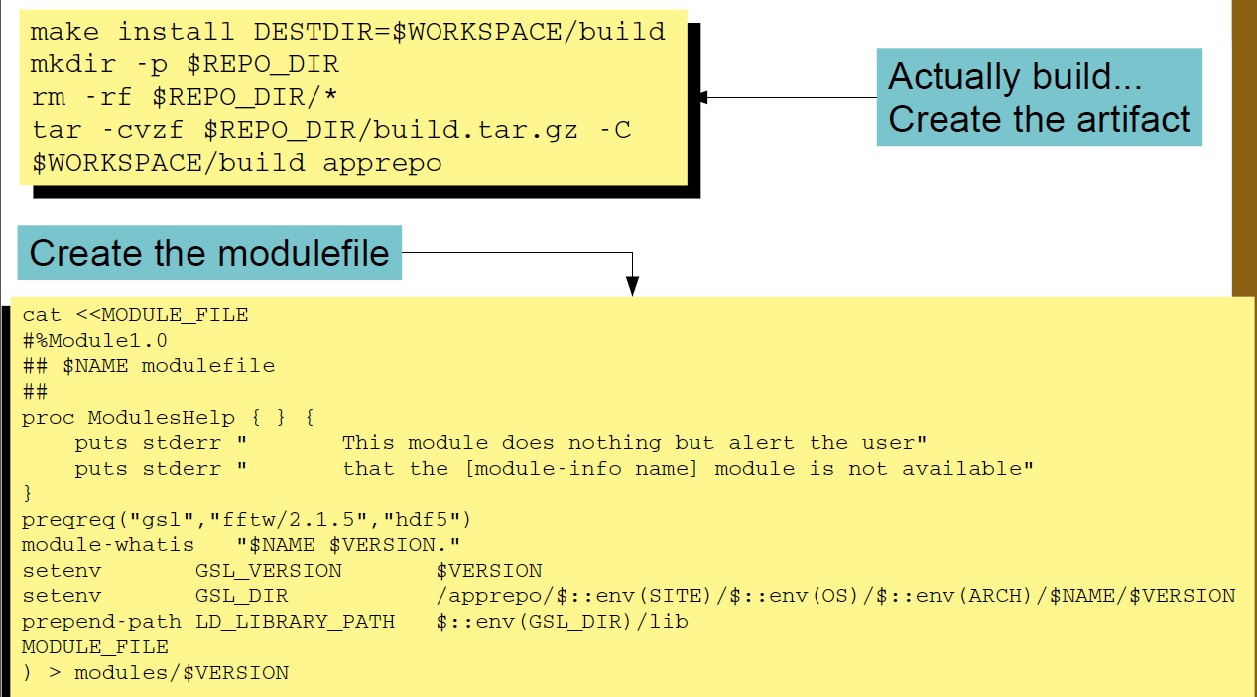
\includegraphics[width=14cm,height=7cm]{build.jpg}
\caption{Installation build script}
\label{fig:build}
\end{figure} 
Figure \ref{fig:build} scripts using modules. \\


The predicted timelines are as follows: 
\begin{enumerate}
\item The month of July will be for Jenkins setup and configurations.
\item August is the study of artefacts creating, suggestions and implementation 
\item September is installation of scientific applications.
\item October is creation of testing bash scripts and gathering results.
\item November is writing of the project report.
\end{enumerate}

% Presented Clearly And Well Organized
% Enough Collected To Test Hypothesis Or Answer Questions
% Student Understands Results (Discussion)
% Student Has Related Results To Research Hypothesis/Question
% Student Has Discussed Limitation(s) Of Own Research
% Student Has Placed Own Work Into Context With Other Research
% Student Has Discussed Own Level Of Contribution

% It is expected that these case studies will lead to insights necessary 
% to provide best-practice guidelines to future development and operation of the service, 
% especially related to optimisation and automation procedures.

% A practical working system is also expected.
\section{Expected Outcome and Conclusion}
The case study of this project indicates that components of the solution already exist and most grid sites administrators have consider them. Jenkins for instance has been inexistence for many years, even before Development Operation design principles were discovered and documented. This leads to be belief that integration of tools is not given a fair chance despite the fact that results will be more than desirable. Traditional installation procedures are still widely used while other e-Infrastructure procedures have evolved, case inpoint, user access. \\

% Challenges
The first step is adopting the correct methodology, the design principles that restructures organisations and changes culture. DevOps completely reinvents the development pipeline from Continuous Integration to Continuous Delivery. The process prides itself for not breaking the ``build process'', but because a great effort is needed to lay the ground work, some processes will have to halt while shifting to the new process. In a short space of time, DevOps requires a personnel to master a number of technologies to fully integrate and automate the development and operations systems together. Not every organisation has the luxury of going through these changes in hopes of achieving better results, especially when they've adapted workarounds to mitigates the effects of inefficiency.  \\

Another major challenge is the usage of Docker. Docker images as artefacts require docker software to be present at each site in-order to execute them. This is not the case in the grid community, not everyone site runs a docker instance. Modulefiles which can be used to achieve the same results of solving dependencies, allows packaging the application using widely used utilities like tar to be artefacts, which can be easily executed on every site. Despite this, Docker cannot be sidelined as it comes with many useful features to enable openness in e-Science. Time has to be spent on each technology looking at the pros and cons and decide on the implementation. \\

% Expected Outcome
The success of this project largely depends on demonstrating a fully automated installation on a grid site. Upon this demonstration, the project would have met all the aims of this research. Tests conducted in the installation process would have been automated by the use of Jenkins platform, complexity of dependencies on applications would have been solved by either using Docker or modulefiles and redistribution of artefacts using CVMFS will not require any work from the site administrators except mounting the repository.  \\ 

The project will lead to new insights necessary to provide best-practice guidelines to future development and operation of services, especially related to optimisation and automation procedures. This will contribute to the knowledge base of e-Science and help solve the general issues plaguing the growth of the field. \\

% Future Work
As stated earlier in this paper, there a number of technologies that can be integrated to achieve our desired solution. In future research, studies of which technologies compliment each other maybe of interests by benchmarking their workflow performance and the degree of difficulty when its comes to integrating them together. The obvious case will be a further study of integrating docker in this project to completely remove the need of modulefiles. \\ 

It is worthwhile to think about security as well. While implementing integration and automation, how is security ensured. Completely removing the human hand to manually approve application for instance pushes projects to rely heavily on security features from these technologies. As DevOps continues to gain popularity in open source, the integration processes may feedback to the designs of these technologies. 

% It Provides A Summary Of The Major Points Of The Proposal
% It Does Summarize The Document
% It Brings Together The Main Points
% It Highlights Most Important Results
% It Makes Clear Student’s Own Contribution
% Some Ideas For Future Work Presented
% Some Discussion Of Other Ways Of Addressing The Same Problem


\bibliography{annot2}

\end{document}